% NOTE:
% latexmk -shell-escape -pvc slides.tex # Watches and compiles on each change.
% latexmk -c slides.tex   # Clean the temporal files.

\documentclass[12pt]{article}

\usepackage{sbc-template}
\usepackage{graphicx,url}
\usepackage[utf8]{inputenc}
\usepackage{babel}
\usepackage{graphicx}
\usepackage{subcaption}
\usepackage{placeins}

% R language listing
% Taken from https://tex.stackexchange.com/questions/110722/trying-to-include-r-code-with-listings-package
\usepackage{color}
\definecolor{dkgreen}{rgb}{0,0.6,0}
\definecolor{gray}{rgb}{0.5,0.5,0.5}
\definecolor{mauve}{rgb}{0.58,0,0.82}
\usepackage{listings}
\renewcommand{\lstlistingname}{Code snippet}
\lstset{ 
  language=R,                     % the language of the code
  basicstyle=\footnotesize,       % the size of the fonts that are used for the code
  numbers=left,                   % where to put the line-numbers
  numberstyle=\tiny\color{gray},  % the style that is used for the line-numbers
  stepnumber=1,                   % the step between two line-numbers. If it's 1, each line
                                  % will be numbered
  numbersep=5pt,                  % how far the line-numbers are from the code
  backgroundcolor=\color{white},  % choose the background color. You must add \usepackage{color}
  showspaces=false,               % show spaces adding particular underscores
  showstringspaces=false,         % underline spaces within strings
  showtabs=false,                 % show tabs within strings adding particular underscores
  frame=single,                   % adds a frame around the code
  rulecolor=\color{black},        % if not set, the frame-color may be changed on line-breaks within not-black text (e.g. commens (green here))
  tabsize=2,                      % sets default tabsize to 2 spaces
  captionpos=b,                   % sets the caption-position to bottom
  breaklines=true,                % sets automatic line breaking
  breakatwhitespace=false,        % sets if automatic breaks should only happen at whitespace
  title=\lstname,                 % show the filename of files included with \lstinputlisting;
                                  % also try caption instead of title
  keywordstyle=\color{blue},      % keyword style
  commentstyle=\color{dkgreen},   % comment style
  stringstyle=\color{mauve},      % string literal style
  escapeinside={\%*}{*)},         % if you want to add a comment within your code
  morekeywords={*,...}            % if you want to add more keywords to the set
} 
%\usepackage{hyperref}

\sloppy
\title{A tool for prioritizing deforestation hotspots in the Brazilian Amazon}

\author{
    Alber Sanchez\inst{1},  
    Guilherme Mataveli\inst{1},  
    Gabriel de Oliveira\inst{2},  
    \\
    Michel E. D. Chaves\inst{1,}\inst{5},  
    Ricardo Dalagnol\inst{3},  
    Fabien H. Wagner\inst{3},  
    \\
    Celso H. L. Silva-Junior\inst{4},  
    Luiz E. O. C. Aragão\inst{1}
}
\address{
    Earth Observation and Geoinformatics Division\\
    National Institute for Space Research - Brazil
    \nextinstitute
    Department of Earth Sciences\\
    University of South Alabama - USA
    \nextinstitute
    Institute of Environment and Sustainability\\
    University of California - USA 
    \nextinstitute
    Program in Biodiversity Conservation\\
    State University of Maranhão - Brazil
    \nextinstitute
    School of Sciences and Engineering\\ 
    São Paulo State University in Tupã - Brazil 
    \email{\{alber.ipia,guilherme.mataveli,luiz.aragao,michel.chaves\}@inpe.br}
    \email{\{wagner.h.fabien,celsohlsj\}@gmail.com}
    \email{deoliveira@southalabama.edu,ricds@hotmail.com}
}


\begin{document} 

\maketitle

\begin{abstract}
Deforestation monitoring and control require scientific tools to increase the impact of official policies under limited resources for environmental law enforcement.
In our paper ``\textit{Science-based Planning Can Support Law Enforcement Actions to Curb Deforestation in the Brazilian Amazon}" we proposed an index for prioritizing deforestation areas for law enforcement.
In this paper, we present an \textsf{R} package that contains both the data and software required to estimate our index.
We expect the public and scientific community to check our proposal along with our tool or to use it as a starting point for improving or proposing creative ways to prioritize areas in the Brazilian Amazon for policy or law enforcement actions.
\end{abstract}
     
\begin{resumo} 
O monitoramento e controle do desmatamento precisam de ferramentas científicas para  aumentar o impacto dos recursos previstos pelas políticas oficiais, para a aplicação da lei ambiental.
Em nosso artigo ``\textit{Science-based Planning Can Support Law Enforcement Actions to Curb Deforestation in the Brazilian Amazon}" propusemos um índice para priorizar áreas de desmatamento, visando subsidiar as ações para aplicação da lei.
Neste artigo, apresentamos um pacote do \textsf{R} que contém os dados e o software necessários para estimar o índice proposto.
Esperamos que o público e a comunidade científica verifiquem nossa proposta, juntamente com nossa ferramenta, ou que a utilizem como ponto de partida para melhorar ou propor formas criativas de priorizar áreas na Amazônia brasileira para ações políticas ou para a aplicação da lei.
\end{resumo}


\section{Introduction}

The deforested area in the Brazilian Amazon is still increasing and has had a positive trend since 2012~\footnote{Deforestation rate in Brazil's Legal Amazon \url{http://terrabrasilis.dpi.inpe.br/app/dashboard/deforestation/biomes/legal_amazon/rates}}. Despite deforestation reduction promises by different administrations, no administration has achieved zero illegal deforestation~\cite{dearealeaopereira2019}.

Deforestation policies and their enforcement are subject to government changes, challenging the establishment of long-term environmental planning. 
Such policies should be subject to public scrutiny and preferably based on scientific principles. 
Therefore, we published a paper entitled \textit{Science-based planning can support law enforcement actions to curb deforestation in the Brazilian Amazon}~\cite{mataveli2022}.
In our paper, we proposed an index for prioritizing areas in the Brazilian Amazon for law enforcement actions. 
This index is based on a set of variables observed during the previous years and aggregated into a regular grid of 25x25 km.
This index was estimated from 2019 to 2022 using the Random Forest algorithm and has been updated for 2023~\cite{mataveli2023}.

To ensure the openness and transparency of our proposal, we prepared a data and software bundle using the \textit{R} language (hereby called package) that allows the public and other research teams to reproduce our methods and findings.
In this paper, we introduce the computational details of the development of the software used to produce our original paper~\cite{mataveli2022}.


\section{Computing environment}

\textit{R} is a programing (scripting) language for statistical computing and graphics~\cite{rlanguage}.
Its source code is open, it runs on the most popular operating systems (GNU/Linux, MacOS, Windows), and it has native support for matrices, linear algebra, and statistical analysis methods~\cite{ihaka1996a}.
\textit{R} is extensible through packages, which enable \textit{R} to load and run code (C, C++, Fortran, Java, Python, or \textit{R}), data, demos, examples, documentation, tests, and consistency checks~\cite{wickham2015}.
\textit{R} also counts with a centralized package repository called CRAN (The Comprehensive R Archive Network) which ensures package availability and a minimal quality level through automated testing and checking.
CRAN counts with almost 20,000 packages, organized in task views, covering topics from actuarial science to Web technologies, including spatial and spatio-temporal analysis of vector and raster geographic data~\cite{Pebesma2012}.
In addition to CRAN, the \textit{R} development community is organized around scientific journals (The \textit{R} Journal, Journal of Statistical Software), blogs (e.g. R-bloggers, The R Blog), and other organizations besides the \textit{R} foundation (Why R foundation, Posit software, rOpenSci, among others).


\section{Scientific reproducibility with \textsf{R}}

The ability to consistently run an experiment setup and obtain similar results has been proposed for some time now and along different areas, causing some confusion regarding the wording used~\cite{plesser2018}.
We adhere to the definitions used by the Association for Computing Machinery (ACM) badging system, which considers three definitions: repeatability, reproducibility, and replicability~\cite{acm2020}.
Repeatability refers to the ability of research teams to reliably repeat their own computations. 
Reproducibility means that independent research teams can obtain the same experimental results using the authors' software artifacts. 
Finally, replicability implies that independent research teams can obtain the same results using their own artifacts.

Given the definitions above, we argue that by using \textit{R} packages, we achieve both repeatability and reproducibility.
For example, we developed the \textit{R} package (see Section~\ref{sec:package}) during the entire development of our manuscript, thus achieving repeatability and, by making it available online, we achieved reproducibility.
Since replicability depends on other research groups collecting their own data and writing their own software, it cannot be achieved by us writing  \textit{R} packages.

\section{Package description}
\label{sec:package}

As mentioned earlier, our \textit{R} package allows users to reproduce the results presented in our paper~\cite{mataveli2022} and its update~\cite{mataveli2023}. 
Our package bundles both the code and the data required to prioritize deforestation areas for 2022 and 2023.
Our package is available at Github\footnote{Prioritize deforestation hotspots \url{https://github.com/albhasan/prioritizedeforestationhotspots}} and has an approximate size of 6 MB (zipped), which unfortunately, disqualifies it from submission to CRAN as it rejects packages larger than 5 MB~\cite{cranpolicy}.

Installing our package requires, in addition to \textsf{R}, the package \textit{devtools}, which allows the installation of packages from GitHub (see Code snippet~\ref{code:install}).

\lstinputlisting[language=R, label={code:install}, caption={Install the package in \textsf{R}. Note that the package \textit{devtools} is required before installation.}]{code/00_install.txt}

This package includes a function to fit the model presented in our paper (\textit{fit\_model}) and a function to estimate its accuracy (\textit{estimate\_accuracy}), which is achieved by adjusting 100 models to the data and then cross-validating them.
An additional function (\textit{results\_to\_shp}) applies thresholds to the results of our model into categories (e.g. low, average, and high) and exports them to a vector file compatible with Geographic Information System software.
Calling these functions reproduces the results presented in our paper (see Code snippet~\ref{code:run}).

These functions take only one parameter, the output directory (\textit{out\_dir}).
After running, the functions store R data files containing the model used to estimate the prioritization index (\textit{final\_model.rds}), the model generated during each iteration of the accuracy estimation (e.g. \textit{param\_final\_100.rds}), and their metrics (e.g. \textit{performance\_test\_100.rds}).
Comma-separated files are also generated containing a summary of the models' root mean square error (\textit{crossvalidation\_tb.csv}), the estimation produced by the final model (\textit{new\_data\_tb.csv}), and an estimation of the importance of each variable in the model (\textit{variable\_importance}.csv). 
In addition, a GeoPackage file is produced (\textit{priority\_classes.gpkg}) containing the prioritization index stored as geographic data compatible with Geographic Information System software (e.g. QGIS or ArcGIS).


\lstinputlisting[language=R, label={code:run}, caption={Reproduce the updated results presented in \cite{mataveli2022}. The resulting files are stored in the directory specified by the variable \textit{out\_dir}.}]{code/01_run.txt}

%The criterion for selecting the best models is their Root Mean Square Error.
% Acho que só de mostrar o que tem no diretorio out_dir e como são organizados já clarificaria muito pra uma pessoa entender o que o pacote faz.

We ran Code snippet~\ref{code:run} using \textsf{R} 4.3.1 running GNU/Linux Ubuntu 20.04.6 (Kernel 5.15.90.1) LTS on top of Windows 10 Subsystem for Linux 1.2.5.0 using 16 of the 32 available cores in a processor Intel Xeon E5-2640 v3 2.593GHz with 32 GB of memory.
The function \textit{fit\_model} took 13 minutes to run
(user 9535.76, system 129.55, elapsed 752.90),  \textit{results\_to\_shp} took 14 hours (user 640670.17, system 10554.66, elapsed 50190.13), and \textit{results\_to\_shp} took a second (user 0.91,  system 0.02, elapsed 0.972).


Our package also includes the data required to run our model: \textit{deforestation\_data} and \textit{deforestation\_grid}.
The former contains the model variables aggregated at 25 km resolution; the latter is the grid itself stored using \textsf{R}'s vector format (an object of the \textit{sf} package~\cite{pebesma2018}).
In addition, our pre-computed results are available as variables. Code snippet~\ref{code:plot_results} shows how to format and plot these results, as shown in Figure~\ref{fig:plot_results_precomputed}.


\begin{figure}[ht]
\centering
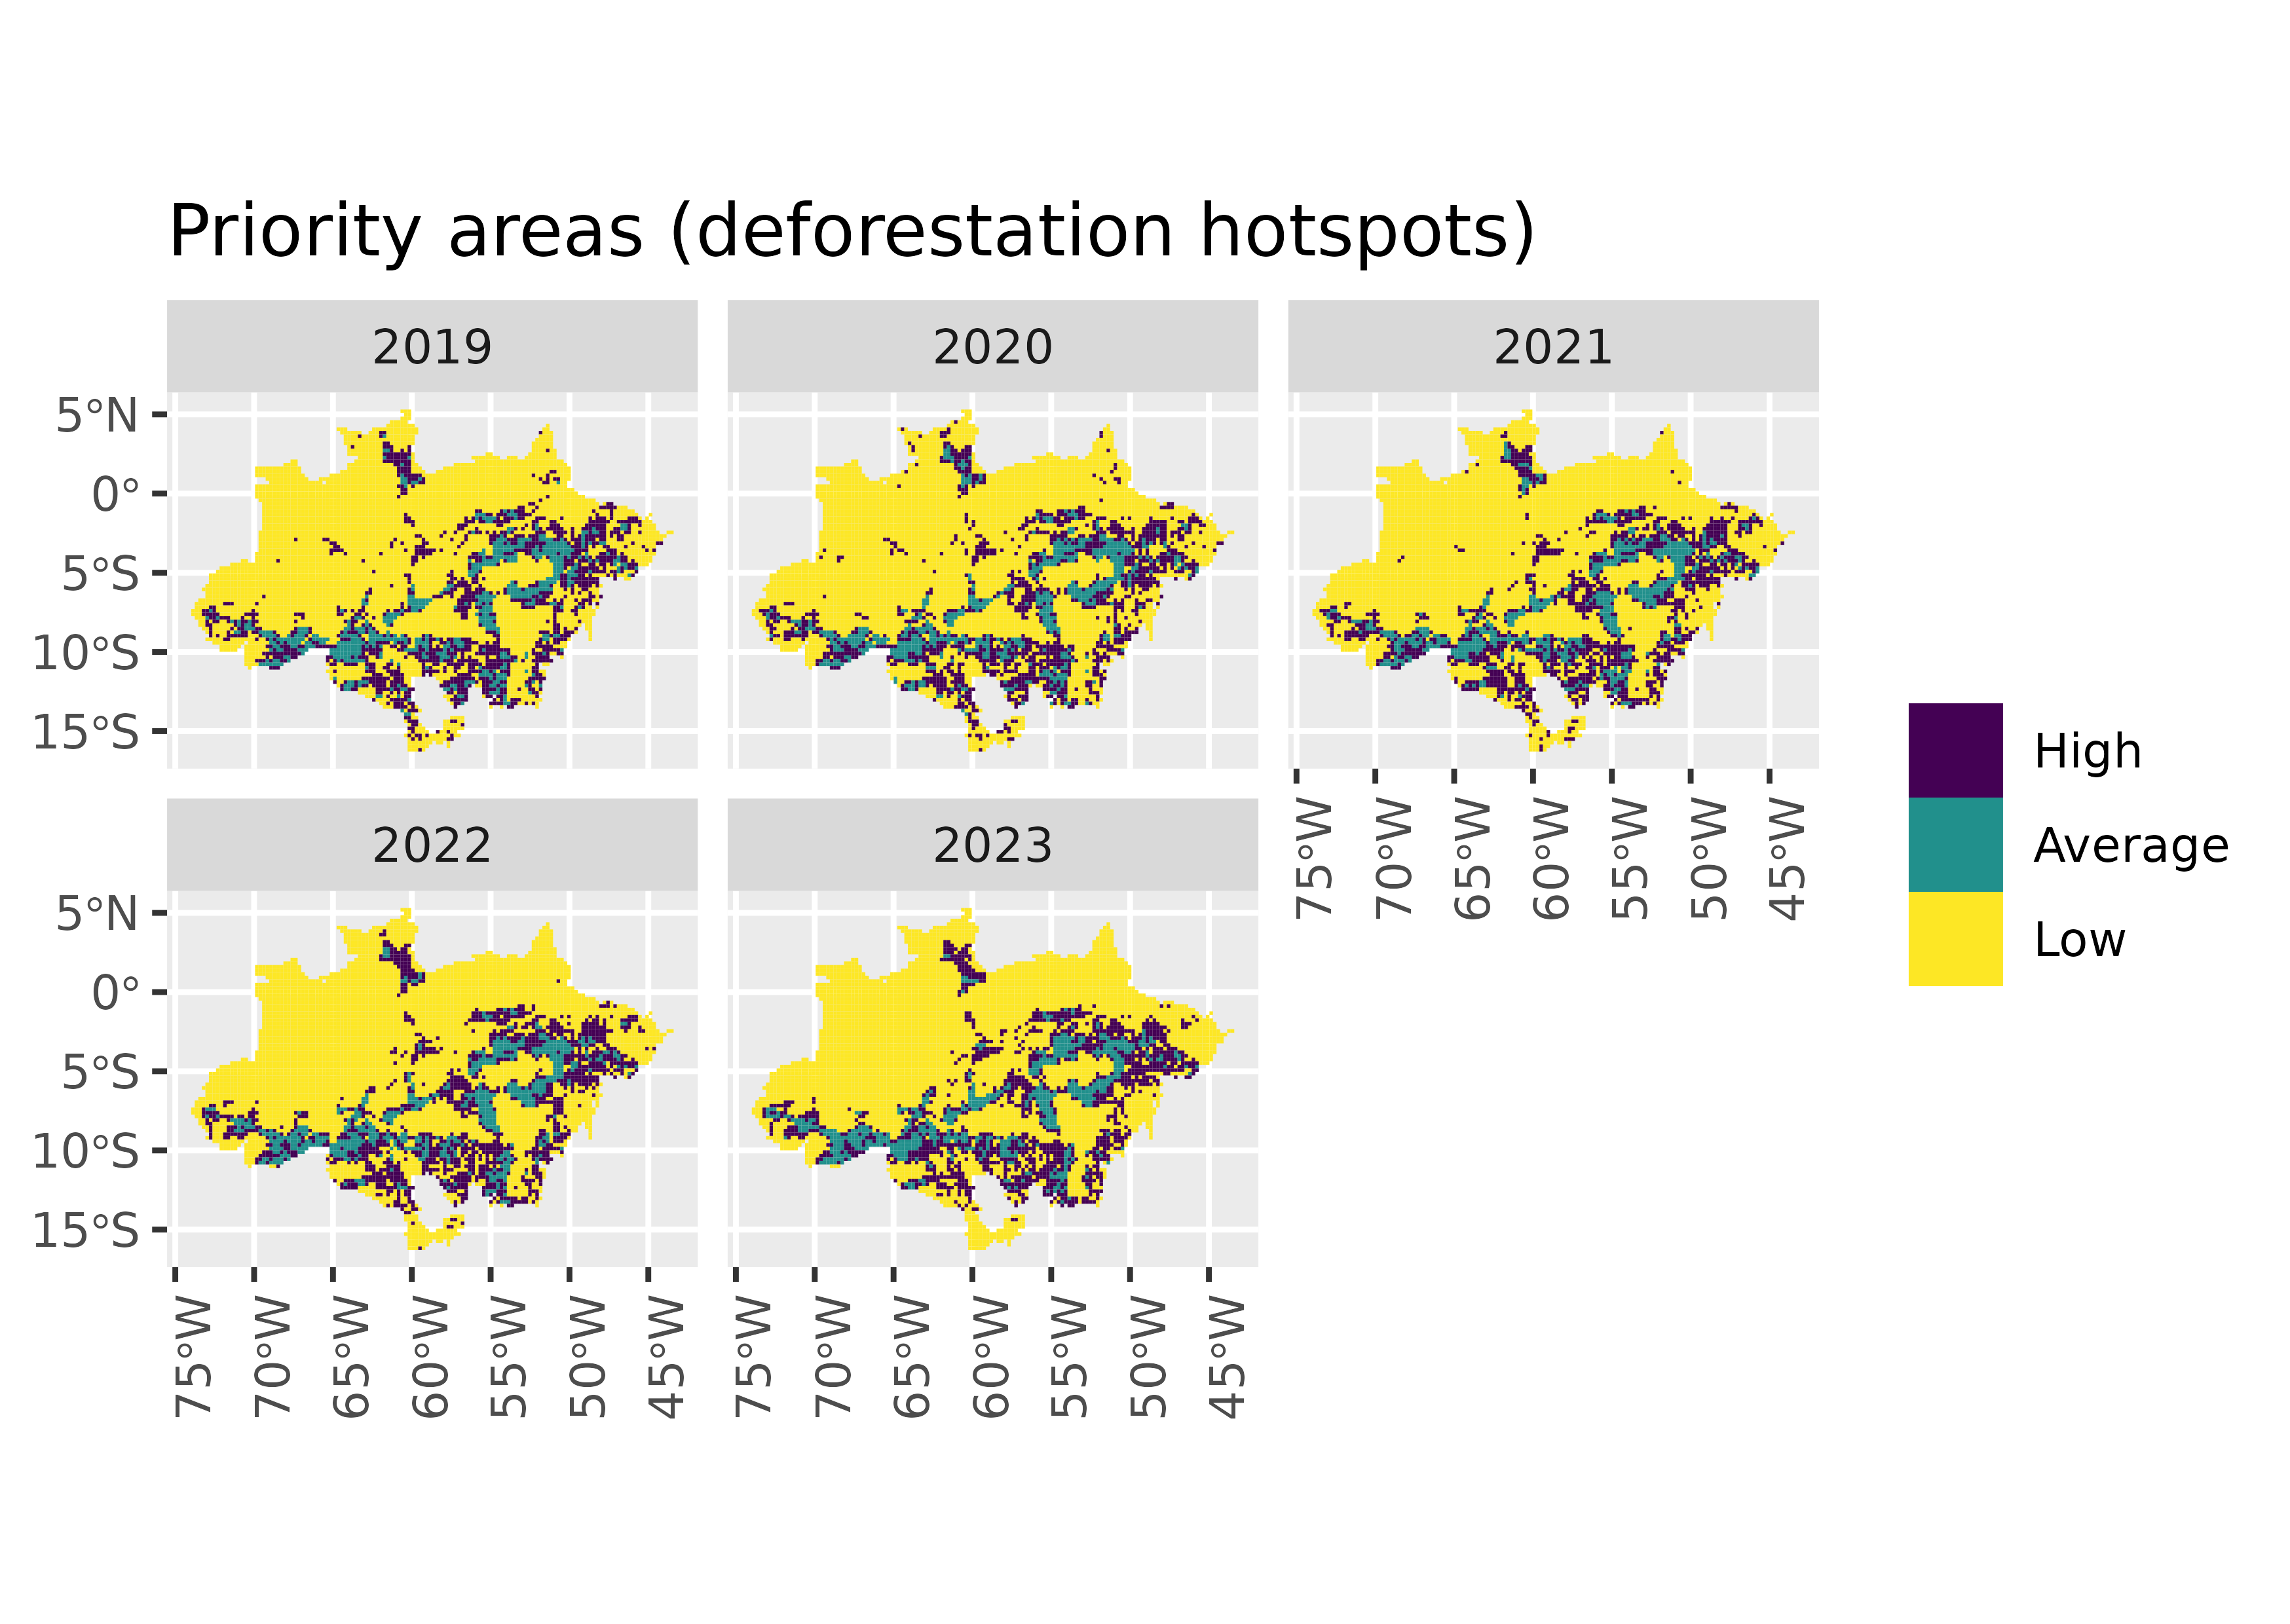
\includegraphics[width=0.8\textwidth,trim={0 1.0cm 0 2.0cm},clip]
{figures/plot_results_precomputed.png}
\caption{Plotting prioritization data stored in the package. This figure is the result of running Code snippet~\ref{code:plot_results}.}
\label{fig:plot_results_precomputed}
\end{figure}

Additional variables for each cell in the grid include an identifier (\textit{id}); a reference year (\textit{ref\_year});  the number of fires the year before the reference year (\textit{active\_fires\_ly}; the area of deforestation during the reference year (\textit{deforestation} in km2) and during one, two, and four years before the reference year ( \textit{def\_1\_ly}, \textit{def\_2\_ly}, and \textit{def\_4\_ly} in km2); and indigenous or protected areas (\textit{area\_PA} in km2).
In addition, the distances to the closest waterway (\textit{dist\_hydro} in km), closest highway (\textit{dist\_road} in km), closest highway or waterway (\textit{dist\_road\_hidro} in km),  and the closest grid centroid with more than 1\% and 2\% deforestation one year before the reference (\textit{dist\_1\_percent\_ly} and  \textit{dist\_2\_percent\_ly}, both in km) are made available.
Code snippet~\ref{code:plot_pas} shows how to plot one of these variables.

\lstinputlisting[language=R, label={code:plot_results}, caption={Plot the results already stored in the package.}]{code/02_plot_results_precomputed.txt}

\lstinputlisting[language=R, label={code:plot_pas}, caption={Plot the extent of protected areas or indigenous lands in each cell in the grid.}]{code/03_plot_pas.txt}


\section{Final remarks}

We presented the \textsf{R} package \textit{prioritizedeforestationhotspots}~\footnote{Prioritize deforestation hotspots \url{https://github.com/albhasan/prioritizedeforestationhotspots}}, which enables users to reproduce the results presented in the paper ``\textit{Science-based Planning Can Support Law Enforcement Actions to Curb Deforestation in the Brazilian Amazon}"~\cite{mataveli2022,mataveli2023}.
This tool comprises not only the software but also the data used during the writing and analysis stages of the aforementioned paper.
In this way, we provide other research teams with the opportunity to check our conclusions and the potential to start extending our research to cover new hypotheses.


\FloatBarrier

\bibliographystyle{sbc}
\bibliography{main}

\end{document}
